In diesem Abschnitt werden sämtliche Vergleichsexperimente unter Verwendung des vollständigen Target-Datensatzes durchgeführt. Dabei umfasst die 
Trainingsmenge etwa 8.000 Datenpunkte, während die Testmenge rund 4.000 Samples beinhaltet.

Verglichen werden drei Netzwerkvarianten: vollständige Netzwerke, Cascade-Netzwerke ohne TF sowie 
Cascade-Netzwerke mit TF. Unter einem vollständgien Netzwerk wird ein Modell verstanden, dessen gesamte Architektur – inklusive 
aller Layer – im Voraus definiert ist und das in einem einzigen Trainingslauf optimiert wird. Dies entspricht dem üblichen Vorgehen beim 
Training klassischer neuronaler Netzwerke.

Es erfolgt ein direkter Vergleich zwischen dem Deep-Cascade-Ansatz, dem Direct-Cascade-Verfahren und dem vollständigen Netzwerkmodell.

\begin{figure}[htpb]
    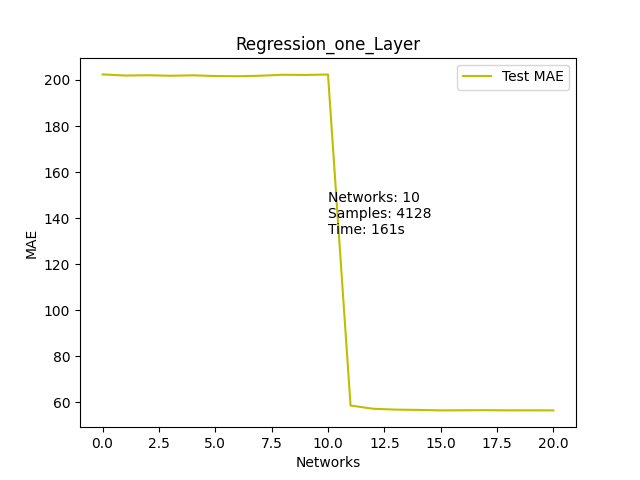
\includegraphics[height=5cm]{../../Plots/ba_plots/regression_large/onelayer_ts.png}
    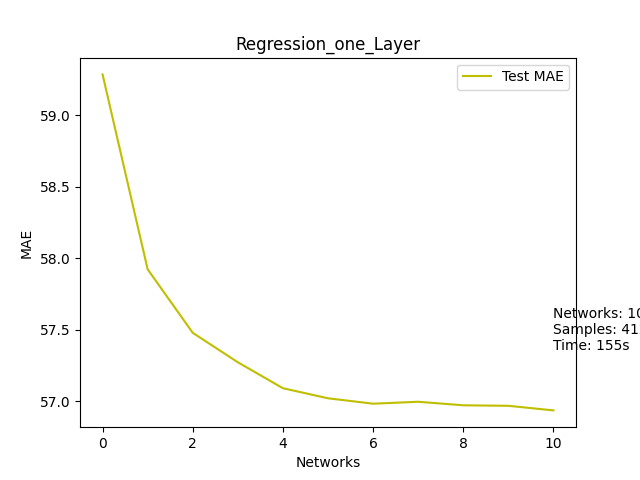
\includegraphics[height=5cm]{../../Plots/ba_plots/regression_large/woonelayer_ts.png}
    \caption{\label{fig:largeregr2} 
    \small{In der Abbildung sind die Ergebnisse der Testläufe 1Lay:TF11/8k/10/21 und 1Lay:8k/10/11 dargestellt. Beide Modelle erreichen am Ende 
    eine vergleichbare Leistung, unterscheiden sich jedoch hinsichtlich der Anzahl an Trainingsdurchläufen bzw. der benötigten Zeit bis zum 
    Erreichen dieses Leistungsniveaus.}}
\end{figure}

Abbildung \ref{fig:largeregr2} zeigt die Ergebnisse des Direct Cascade-Verfahrens. Die linke Seite stellt die Variante mit TF dar. Es fällt auf, 
dass bei vielen Target-Daten das direkte Training auf den Target-Daten zu besseren Ergebnissen führt, da das vom Source-Datensatz 
übertragene Wissen oftmals weniger gut auf die Target-Daten übertragbar ist. Dieser Effekt tritt jedoch nur bei ausreichender Verfügbarkeit 
von Target-Daten auf. Im Vergleich dazu erzielen auch die Deep Cascade-Modelle vergleichbare Ergebnisse. Ein vollständig trainiertes Netzwerk, 
wie in Abbildung \ref{fig:largeregr2comp} dargestellt, erreicht eine ähnliche Performanz wie die beiden Kaskadenversionen.

\begin{figure}[htpb]
    \centering
    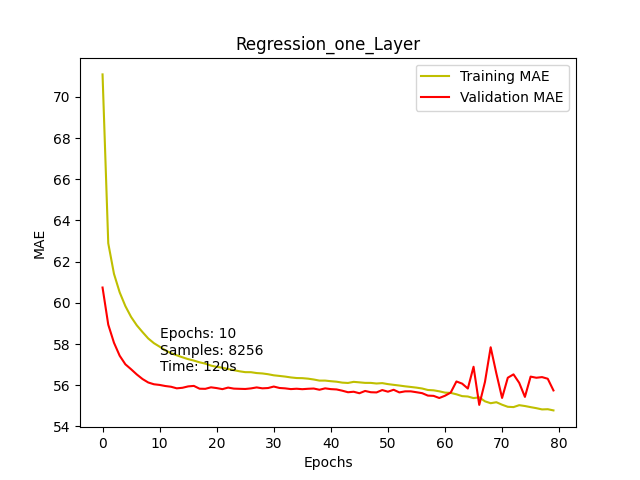
\includegraphics[height=5cm]{../../Plots/ba_plots/regression_large/onelayer_complete.png}
    \caption{\label{fig:largeregr2comp} 
    \small{Bei dem vorliegenden Modell handelt es sich um den Test 1Lay:Comp/8k//8. Dieser wurde unter Verwendung einer großen Menge an Target-Daten direkt 
    trainiert, weshalb die erzielten Ergebnisse im weiteren Verlauf als Referenz für die bestmögliche Leistung herangezogen werden.}}
\end{figure}

Dies ist darauf zurückzuführen, dass die lineare Aktivierungsfunktion sowie der MSE Loss im Kontext der Kaskadierung keine 
negativen Effekte verursachen. Dementsprechend erzielt die Regression mit Kaskadennetzwerken eine deutlich bessere Leistung als die 
Klassifikation, da sie nahe an die Ergebnisse eines vollständig trainierten Netzwerks heranreicht – ein Effekt, der bei Klassifikationsaufgaben 
bisher nicht beobachtet wurde.

Da das Netzwerk vergleichbare Ergebnisse mit TF erzielt, kann davon ausgegangen werden, dass der Einsatz von TF in diesem Fall 
erfolgreich war.
